\chapter{Las leyes de Newton de la dinámica}\label{ch:b1:newton-dynamics}

Un paracaidista sale del avión y, en una docena de segundos, deja de
acelerar: a doscientos kilómetros por hora el aire empuja exactamente
tanto como tira la Tierra. Un coche toma una curva demasiado deprisa y los
neumáticos ceden; un camión en una carretera de montaña avanza a paso lento
en una marcha corta, sostenido por el mismo rozamiento que le permite
detenerse en llano. La cinemática describía movimientos; la dinámica los
explica, a partir de una única ley que liga la aceleración de un cuerpo con
las \omterm{def:b1:newton-dynamics:momentum}{fuerzas} que actúan sobre él. Este capítulo enuncia las tres \omterm{thm:b1:newton-dynamics:laws}{leyes de
Newton}, cataloga las \omterm{def:b1:newton-dynamics:momentum}{fuerzas} que aparecen al nivel de este volumen ---
peso, resortes, hilos, contactos, \omterm{prop:b1:newton-dynamics:friction}{rozamiento seco} y fluido --- y muestra
cómo pasar de un dibujo de las \omterm{def:b1:newton-dynamics:momentum}{fuerzas} a una ecuación diferencial y a su
solución.

\begin{omfigure}
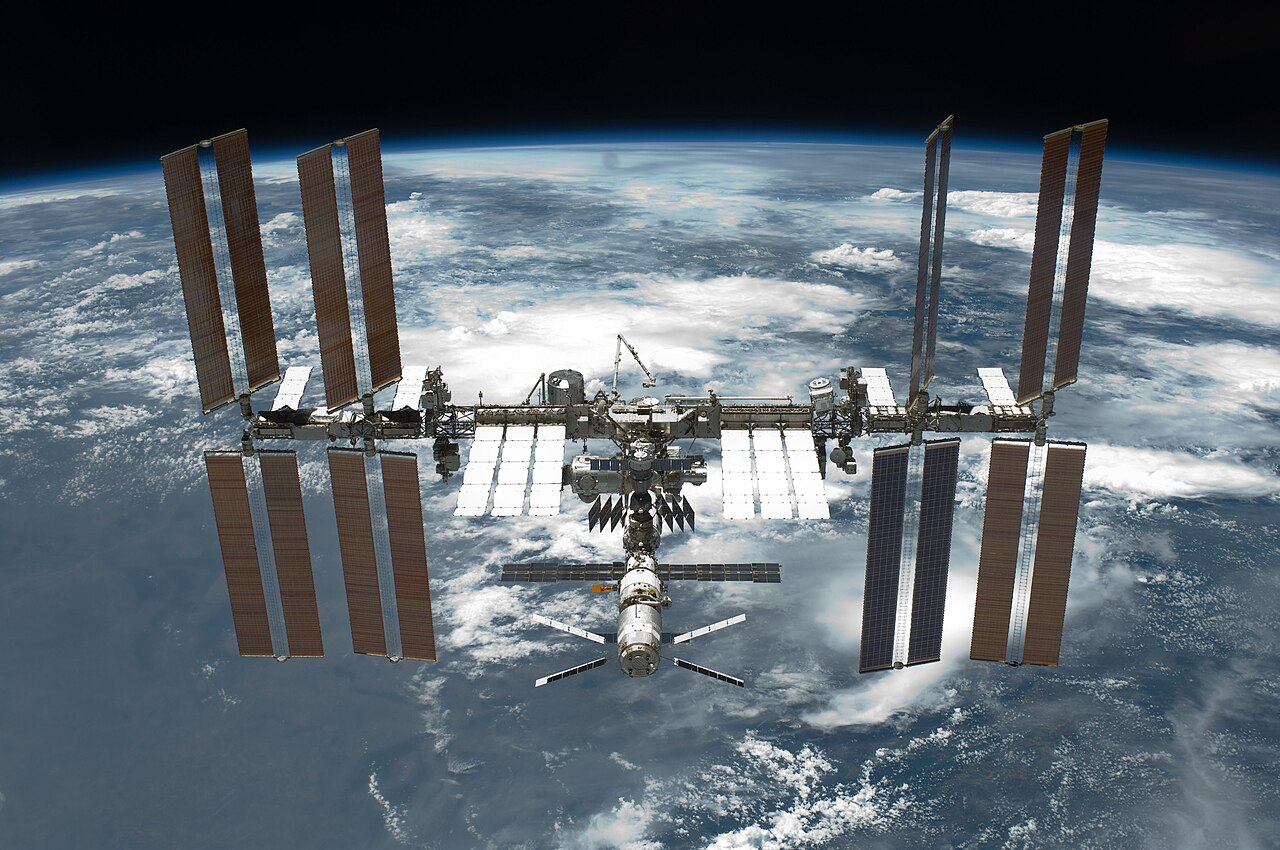
\includegraphics[width=0.60\linewidth]{images/book3/iss-orbit.jpg}

{\small La Estación Espacial Internacional vista desde el transbordador que se aleja (NASA): todo lo que hay a bordo está en caída libre a la vez, y por eso nada a bordo parece pesar.}
\end{omfigure}

\section{Masa, cantidad de movimiento y las tres leyes}

\begin{definition}[Masa, cantidad de movimiento, fuerza]\label{def:b1:newton-dynamics:momentum}
\index{masa}\index{cantidad de movimiento}\index{fuerza}
Un \omterm{def:b1:point-kinematics:frame}{punto material} tiene una \emph{masa inercial} $m > 0$ (kilogramos), una
medida de su resistencia a los cambios de velocidad, independiente del
\omterm{def:b1:point-kinematics:frame}{sistema de referencia}. Su \emph{cantidad de movimiento} en un sistema es
\[
\vect p = m\,\vect v \qquad (\unit{kg.m/s}).
\]
Una \emph{fuerza} $\vect F$ (newtons) es la acción de otro cuerpo sobre el
punto; las fuerzas se suman como vectores, y la \emph{resultante} es su
suma $\sum\vect F$.
\end{definition}

\begin{theorem}[Leyes de Newton]\label{thm:b1:newton-dynamics:laws}
\index{leyes de Newton}\index{sistema inercial}\index{principio de inercia}\index{acción y reacción}
\begin{enumerate}
  \item \emph{\omterm{thm:b1:newton-dynamics:laws}{Principio de inercia}.} Existen \omterm{def:b1:point-kinematics:frame}{sistemas de referencia},
        llamados \emph{inerciales} (o galileanos), en los que un \omterm{def:b1:point-kinematics:frame}{punto
        material} sin \omterm{def:b1:newton-dynamics:momentum}{fuerzas}, o con \omterm{def:b1:newton-dynamics:momentum}{fuerzas} de resultante nula, se mueve
        en línea recta con velocidad constante. Todo sistema en traslación
        rectilínea uniforme respecto de un \omterm{thm:b1:newton-dynamics:laws}{sistema inercial} es inercial.
  \item \emph{Ley de la \omterm{def:b1:newton-dynamics:momentum}{cantidad de movimiento}.} En un \omterm{thm:b1:newton-dynamics:laws}{sistema inercial},
        \[
        \frac{\dd\vect p}{\dd t} = \sum\vect F, \qquad \text{es decir}\qquad
        m\,\vect a = \sum\vect F \ \text{ para una masa constante } m .
        \]
  \item \emph{\omterm{thm:b1:newton-dynamics:laws}{Acción y reacción}.} Si el cuerpo $A$ ejerce $\vect F_{A\to B}$
        sobre el cuerpo $B$, entonces $B$ ejerce $\vect F_{B\to A} = -\vect F_{A\to B}$
        sobre $A$, a lo largo de la recta que los une.
\end{enumerate}
\end{theorem}
\admitted

\begin{remark}[Qué dicen las leyes]\label{rem:b1:newton-dynamics:meaning}
La primera ley no es un caso particular de la segunda: \emph{define} los
sistemas en los que vale la segunda. En la práctica, un laboratorio en la
Tierra es inercial con excelente precisión para experimentos que duran
minutos (\cref{ch:b1:non-inertial-frames} cuantifica el error); un sistema
ligado al Sol y a las estrellas lejanas lo es todavía más. La segunda ley
es una ecuación vectorial: tres ecuaciones escalares, una por eje, y la
elección de ejes (\cref{ch:b1:point-kinematics}) es la primera decisión de
todo problema. La tercera ley vale en cada instante para las \omterm{def:b1:newton-dynamics:momentum}{fuerzas} de
contacto y gravitatorias de este volumen.
\end{remark}

\begin{definition}[Sistema cerrado; conservación de la cantidad de movimiento]\label{def:b1:newton-dynamics:conservation}
\index{sistema cerrado}\index{conservación de la cantidad de movimiento}
Un \emph{sistema cerrado} no intercambia materia con el exterior. Para un
sistema de \omterm{def:b1:point-kinematics:frame}{puntos materiales}, las \omterm{def:b1:newton-dynamics:momentum}{fuerzas} internas se cancelan por parejas
(tercera ley), y la \omterm{def:b1:newton-dynamics:momentum}{cantidad de movimiento} total $\vect P = \sum m_i\vect v_i$
obedece $\dd\vect P/\dd t = \sum\vect F_{\mathrm{ext}}$: se conserva cuando
se anulan las \omterm{def:b1:newton-dynamics:momentum}{fuerzas} exteriores (\cref{ch:b1:systems-of-points} lo
desarrolla).
\end{definition}

\section{Las fuerzas habituales}

\begin{proposition}[Peso y gravitación]\label{prop:b1:newton-dynamics:weight}
\index{peso}\index{campo gravitatorio}
Cerca de la superficie terrestre, un cuerpo de \omterm{def:b1:newton-dynamics:momentum}{masa} $m$ es atraído por su
\emph{peso} $\vect P = m\vect g$, donde $\vect g$ es el \omterm{prop:b1:newton-dynamics:weight}{campo gravitatorio}
local, $g \approx \qty{9.81}{m/s^2}$, dirigido hacia abajo (hacia el
centro, con muy buena aproximación). Más en general, una \omterm{def:b1:newton-dynamics:momentum}{masa} $M$ a
distancia $r$ atrae a $m$ con $\vect F = -GMm/r^2\,\vect e_r$
(\cref{ch:b1:central-forces}); en la superficie de una esfera de radio
$R$, $g = GM/R^2$. Obsérvese la unidad: \unit{N/kg} y \unit{m/s^2} son la
misma, y por eso todos los cuerpos caen igual.
\end{proposition}

\begin{proof}
La ley de gravitación de Newton se admite y se explora en
\cref{ch:b1:central-forces}; $g = GM/R^2 = 6.67\times10^{-11} \times
5.97\times10^{24}/(6.37\times10^6)^2 = \qty{9.8}{m/s^2}$.
\end{proof}

\begin{proposition}[Resorte; hilo]\label{prop:b1:newton-dynamics:springstring}
\index{ley de Hooke}\index{resorte}\index{tensión}
Un resorte ideal de constante de rigidez $k$ y longitud natural $\ell_0$,
estirado hasta la longitud $\ell$ a lo largo del vector unitario $\vect u$
que va de su extremo fijo al cuerpo, ejerce sobre este la \emph{\omterm{def:b1:newton-dynamics:momentum}{fuerza} recuperadora}
\[
\vect F = -k(\ell - \ell_0)\,\vect u \qquad (\text{ley de Hooke}),
\]
dirigida hacia su longitud natural. Un hilo ideal (sin \omterm{def:b1:newton-dynamics:momentum}{masa} e
inextensible) ejerce una \emph{tensión} $\vect T$ a lo largo de sí mismo,
tirando, con el mismo módulo en los dos extremos y en toda su longitud
(incluso pasando por una polea sin \omterm{def:b1:newton-dynamics:momentum}{masa} ni rozamiento).
\end{proposition}

\begin{proof}
La \omterm{prop:b1:newton-dynamics:springstring}{ley de Hooke} es un modelo empírico válido para deformaciones pequeñas.
El hilo: un elemento sin \omterm{def:b1:newton-dynamics:momentum}{masa} cumple $0 = \vect T_1 + \vect T_2$ por la
segunda ley de Newton, luego la tensión se transmite sin cambio.
\end{proof}

\begin{proposition}[Fuerzas de contacto: reacción normal y rozamiento seco]\label{prop:b1:newton-dynamics:friction}
\index{reacción normal}\index{rozamiento seco}\index{leyes de Coulomb del rozamiento}\index{coeficiente de rozamiento}
Una superficie sólida ejerce sobre un cuerpo que la toca una
\emph{\omterm{prop:b1:newton-dynamics:friction}{reacción normal}} $\vect N$, perpendicular a la superficie y
repulsiva ($N \geq 0$: una superficie no puede tirar), y una \emph{\omterm{def:b1:newton-dynamics:momentum}{fuerza}
de rozamiento} tangencial $\vect T$. Leyes de Coulomb: si el cuerpo no
desliza, $\abs{\vect T} \leq \mu_s N$ (el rozamiento \emph{estático} se
ajusta a lo que haga falta, hasta ese límite); si desliza con velocidad
$\vect v_g$ respecto de la superficie,
$\vect T = -\mu_d N\,\vect v_g/\abs{\vect v_g}$ (rozamiento
\emph{cinético}, que se opone al deslizamiento), con $\mu_d \leq \mu_s$
coeficientes del orden de $0.1$ a $1$ según los materiales, e
independientes del área de contacto y de la rapidez.
\end{proposition}
\admitted

\begin{omfigure}
\begin{tikzpicture}[font=\small, x=1cm, y=1cm]
  % incline
  \draw[thick] (0,0) -- (6,0) -- (0,3.0) -- cycle;
  \node at (4.8,0.32) {$\alpha$};
  \draw (6,0) ++(-1.2,0) arc (180:153.4:1.2);
  % block center on incline at x=3: surface point (3,1.5); normal direction (0.447,0.894) ; block square rotated 26.6 deg, approximate with a rotated rectangle
  \begin{scope}[shift={(3,1.5)}, rotate=-26.6]
    \draw[thick, fill=omDef!15] (-0.5,0) rectangle (0.5,0.7);
    \coordinate (G) at (0,0.35);
  \end{scope}
  \fill (G) circle (1.4pt);
  \draw[-Stealth, omThm, very thick] (G) -- ++(0,-1.6) node[below] {$m\vect g$};
  \draw[-Stealth, omDef, very thick] (G) -- ++(0.447*1.43,0.894*1.43) node[above right] {$\vect N$};
  \draw[-Stealth, omProp, very thick] (G) -- ++(-0.894*0.9,0.447*0.9) node[left] {$\vect T$};
  \draw[-Stealth] (5.0,2.2) -- ++(0.894*0.9,-0.447*0.9) node[right] {$x$};
  \draw[-Stealth] (5.0,2.2) -- ++(0.447*0.9,0.894*0.9) node[above] {$y$};
\end{tikzpicture}\qquad
\begin{tikzpicture}
\begin{axis}[omaxis, width=6.6cm, height=4.6cm, xlabel={fuerza aplicada $F$}, ylabel={rozamiento $T$},
    xmin=0, xmax=3.2, ymin=0, ymax=2.2, xtick={1.5}, xticklabels={$\mu_sN$}, ytick={1.2,1.5}, yticklabels={$\mu_dN$,$\mu_sN$}]
  \addplot[omDef, thick, domain=0:1.5, samples=2] {x};
  \addplot[omThm, thick, domain=1.5:3.2, samples=2] {1.2};
  \draw[dashed, omExo] (axis cs:1.5,0) -- (axis cs:1.5,1.5);
  \node[omDef, font=\footnotesize, anchor=west] at (axis cs:0.15,1.75) {en reposo: $T = F$};
  \node[omThm, font=\footnotesize, above] at (axis cs:2.4,1.2) {deslizando: $T = \mu_dN$};
\end{axis}
\end{tikzpicture}

{\small Izquierda: las \omterm{def:b1:newton-dynamics:momentum}{fuerzas} sobre un bloque en un plano inclinado ---
peso, \omterm{prop:b1:newton-dynamics:friction}{reacción normal} y rozamiento a lo largo de la superficie --- y los
ejes naturales. Derecha: las leyes de Coulomb: en reposo el rozamiento
equilibra la \omterm{def:b1:newton-dynamics:momentum}{fuerza} aplicada hasta $\mu_sN$; en cuanto empieza el
deslizamiento cae a $\mu_dN$ y ahí se queda.}
\end{omfigure}

\begin{proposition}[Rozamiento fluido]\label{prop:b1:newton-dynamics:drag}
\index{rozamiento fluido}\index{fuerza de arrastre}\index{ley de Stokes}
Un cuerpo que se mueve con velocidad $\vect v$ en un fluido en reposo
siente una \emph{\omterm{prop:b1:newton-dynamics:drag}{fuerza de arrastre}} opuesta a $\vect v$: a baja rapidez
(tamaño pequeño, fluido viscoso) es lineal, $\vect F = -\alpha\vect v$
--- para una esfera de radio $r$ en un fluido de viscosidad $\eta$,
$\alpha = 6\pi\eta r$ (Stokes); a rapidez alta (cuerpos grandes y rápidos
en aire o agua) es cuadrática,
\[
\vect F = -\tfrac12\,\rho\,C_xS\,v\,\vect v ,
\]
con $\rho$ la densidad del fluido, $S$ la sección del cuerpo enfrentada al
flujo y $C_x$ un \emph{coeficiente de arrastre} \omterm{def:b1:units-dimensions:dimension}{adimensional} ($0.5$ para
una esfera, $0.3$ para un coche, $1$ para un disco plano). El número de
Reynolds $\rho vL/\eta$ (\cref{rem:b1:units-dimensions:pi}) decide: lineal
por debajo de $1$, cuadrático por encima de unos $1000$.
\end{proposition}
\admitted

\begin{remark}[Otras fuerzas]\label{rem:b1:newton-dynamics:others}
El empuje de Arquímedes es una resultante de \omterm{def:b1:newton-dynamics:momentum}{fuerzas} de presión, deducida
en \cref{ch:b1:fluid-statics}; las \omterm{def:b1:newton-dynamics:momentum}{fuerzas} eléctrica y magnética sobre una
carga son el objeto de \cref{ch:b1:charged-particles}. Todas las \omterm{def:b1:newton-dynamics:momentum}{fuerzas}
de este capítulo son \emph{modelos} de interacciones de contacto o de
campo, válidos dentro de límites declarados --- el resorte de Hooke se
rompe, el rozamiento de Coulomb falla a presiones altas y el arrastre de
Stokes falla a rapidez alta. Parte de toda solución es comprobar que el
modelo empleado se aplica.
\end{remark}

\section{Resolver un problema de dinámica}

\begin{method}[De la situación a la ecuación]\label{met:b1:newton-dynamics:method}
\begin{enumerate}
  \item \emph{Sistema}: nómbrese el cuerpo tratado como punto.
  \item \emph{\omterm{def:b1:point-kinematics:frame}{Sistema de referencia}}: nómbrese y compruébese que es
        inercial (o trátese como tal con la precisión exigida).
  \item \emph{\omterm{def:b1:newton-dynamics:momentum}{Fuerzas}}: enumérese todo cuerpo que toque o atraiga al
        sistema y dibújese cada \omterm{def:b1:newton-dynamics:momentum}{fuerza} en un esquema (el diagrama de
        \omterm{def:b1:newton-dynamics:momentum}{fuerzas}); nada más interviene.
  \item \emph{Coordenadas}: elíjanse ejes adaptados al movimiento
        (\cref{met:b1:point-kinematics:choose}) y exprésese $\vect a$.
  \item \emph{Proyéctese} $m\vect a = \sum\vect F$ sobre los ejes; úsense
        las ligaduras (un cuerpo sobre una superficie permanece en ella:
        $a_\perp = 0$; un hilo de longitud fija: igual rapidez en los dos
        extremos).
  \item \emph{Resuélvase} y \emph{compruébese}: dimensiones, casos
        límite, signos ($N \geq 0$, $\abs T \leq \mu_sN$ si está en reposo).
\end{enumerate}
\end{method}

\begin{example}[Bloque en un plano inclinado]\label{ex:b1:newton-dynamics:incline}
Bloque de \omterm{def:b1:newton-dynamics:momentum}{masa} $m$ en un plano inclinado un ángulo $\alpha$, con
coeficientes $\mu_s$ y $\mu_d$. Ejes: $x$ pendiente abajo, $y$ según la
normal. Peso $(mg\sin\alpha, -mg\cos\alpha)$, reacción $(0, N)$,
rozamiento $(-T, 0)$ si desliza hacia abajo. Según $y$: $N = mg\cos\alpha$.
En reposo, según $x$: $T = mg\sin\alpha \leq \mu_sN = \mu_smg\cos\alpha$,
es decir $\tan\alpha
\leq \mu_s$: el bloque aguanta hasta el ángulo $\arctan\mu_s$ --- una
medida de $\mu_s$ que no necesita balanza. Deslizando: $ma = mg\sin\alpha -
\mu_dmg\cos\alpha$, luego $a = g(\sin\alpha - \mu_d\cos\alpha)$, con
independencia de $m$: \qty{3.2}{m/s^2} para $\alpha = 30^\circ$ y $\mu_d = 0.2$.
\end{example}

\begin{example}[El péndulo simple]\label{ex:b1:newton-dynamics:pendulum}
\index{péndulo simple}
\omterm{def:b1:newton-dynamics:momentum}{Masa} $m$ en un hilo de longitud $\ell$, con ángulo $\theta$ respecto de la
vertical descendente. \omterm{def:b1:point-kinematics:cylindrical}{Coordenadas polares} en el punto de suspensión: $\vect a =
-\ell\dot\theta^2\,\vect e_r + \ell\ddot\theta\,\vect e_\theta$; \omterm{def:b1:newton-dynamics:momentum}{fuerzas}:
el peso $mg(\cos\theta\,\vect e_r - \sin\theta\,\vect e_\theta)$ y la
tensión $-T\vect e_r$. Según $\vect e_\theta$: $m\ell\ddot\theta =
-mg\sin\theta$,
\[
\ddot\theta + \frac{g}{\ell}\sin\theta = 0 ,
\]
que para ángulos pequeños ($\sin\theta \approx \theta$) es la ecuación
armónica con $\omega_0 = \sqrt{g/\ell}$: periodo $T_0 = 2\pi\sqrt{\ell/g}$,
el $k = 2\pi$ que \cref{ex:b1:units-dimensions:pendulum} no podía
proporcionar. Según $\vect e_r$: $T = mg\cos\theta + m\ell\dot\theta^2$ ---
el hilo tira con más \omterm{def:b1:newton-dynamics:momentum}{fuerza} abajo, donde la rapidez es mayor.
\end{example}

\begin{omfigure}
\begin{tikzpicture}[font=\small, x=1cm, y=1cm]
  \draw[thick] (-1,3.2) -- (1,3.2); \fill[pattern=north east lines] (-1,3.2) rectangle (1,3.45);
  \fill (0,3.2) circle (1.2pt);
  \draw[dashed] (0,3.2) -- (0,0.2);
  \coordinate (M) at ($(0,3.2)+(-65:2.8)$);
  \draw[thick] (0,3.2) -- (M);
  \fill[omDef] (M) circle (3pt); \node[below right] at (M) {$m$};
  \draw (0,2.3) arc (-90:-65:0.9); \node at (0.25,2.05) {$\theta$};
  \draw[-Stealth, omThm, very thick] (M) -- ++(0,-1.3) node[below] {$m\vect g$};
  \draw[-Stealth, omDef, very thick] (M) -- ++(115:1.6) node[pos=0.55, left, xshift=-2pt] {$\vect T$};
  \draw[-Stealth, omProp, thick] (M) -- ++(-65:0.9) node[right] {$\vect e_r$};
  \draw[-Stealth, omProp, thick] (M) -- ++(25:0.9) node[right] {$\vect e_\theta$};
  \draw[omDef!40] ($(0,3.2)+(-110:2.8)$) arc (-110:-60:2.8);
\end{tikzpicture}\qquad
\begin{tikzpicture}
\begin{axis}[omaxis, axis x line=bottom, width=7.2cm, height=4.8cm, xlabel={$t/\tau$}, ylabel={$v/v_\infty$},
    xmin=0, xmax=5, ymin=0, ymax=1.2, ytick={0.5,1}, xtick={1,2,3,4,5}]
  \addplot[omDef, thick, domain=0:5, samples=100] {1 - exp(-x)};
  \addplot[omThm, thick, domain=0:5, samples=100] {tanh(x)};
  \addplot[omExo, dashed, domain=0:5, samples=2] {1};
  \node[omDef, font=\footnotesize] at (axis cs:3.6,0.8) {arrastre lineal};
  \node[omThm, font=\footnotesize] at (axis cs:1.2,1.1) {arrastre cuadrático};
\end{axis}
\end{tikzpicture}

{\small Izquierda: el \omterm{ex:b1:newton-dynamics:pendulum}{péndulo simple}, sus dos \omterm{def:b1:newton-dynamics:momentum}{fuerzas} y la base polar
usada para proyectar la ley de Newton. Derecha: un cuerpo que cae desde el
reposo bajo su peso y una \omterm{prop:b1:newton-dynamics:drag}{fuerza de arrastre}: la rapidez tiende a la
\omterm{prop:b1:newton-dynamics:terminal}{velocidad límite} $v_\infty$, de forma exponencial con arrastre lineal
($\tau = m/\alpha$) y como una tangente hiperbólica con arrastre
cuadrático ($\tau = v_\infty/g$).}
\end{omfigure}

\begin{proposition}[Caída con arrastre; velocidad límite]\label{prop:b1:newton-dynamics:terminal}
\index{velocidad límite}
Un cuerpo de \omterm{def:b1:newton-dynamics:momentum}{masa} $m$ que cae desde el reposo bajo su peso y una \omterm{prop:b1:newton-dynamics:drag}{fuerza de
arrastre} alcanza una \emph{\omterm{prop:b1:newton-dynamics:terminal}{velocidad límite}} en la que ambas se
equilibran. Arrastre lineal: $m\dot v = mg - \alpha v$,
$v = v_\infty(1 - \eu^{-t/\tau})$ con $v_\infty = mg/\alpha$,
$\tau = m/\alpha$. Arrastre cuadrático: $m\dot v = mg -
\tfrac12\rho C_xSv^2$, $v = v_\infty\tanh(t/\tau)$ con
\[
v_\infty = \sqrt{\frac{2mg}{\rho C_xS}}, \qquad \tau = \frac{v_\infty}{g} .
\]
\end{proposition}

\begin{proof}
Lineal: una ecuación de primer orden, $\tau\dot v + v = v_\infty$
(\cref{thm:b1:transient-regimes:firstorder}). Cuadrática: con
$u = v/v_\infty$, $\dot u = (1 - u^2)/\tau$; separando variables,
$\int\dd u/(1 - u^2) = \operatorname{artanh}u = t/\tau$ (la fracción
racional $1/(1 - u^2) = \tfrac12[1/(1 - u) + 1/(1 + u)]$ se integra a
$\tfrac12\ln\frac{1 + u}{1 - u}$), de donde $u = \tanh(t/\tau)$.
\end{proof}

\begin{example}[Dos velocidades límite]\label{ex:b1:newton-dynamics:terminal}
Un paracaidista, $m = \qty{80}{kg}$, boca abajo, $C_xS \approx \qty{0.8}{m^2}$
en el aire ($\rho = \qty{1.2}{kg/m^3}$): $v_\infty = \sqrt{2 \times 785/(1.2
\times 0.8)} = \qty{40}{m/s}$, alcanzada (al $90\%$) en unos $1.5\tau =
\qty{6}{s}$. Una gotita de niebla, $r = \qty{10}{\micro m}$, en régimen de
Stokes ($\eta_{\text{aire}} = \qty{1.8e-5}{Pa.s}$): $v_\infty = mg/6\pi\eta r =
\qty{1.2}{cm/s}$ --- por eso la niebla se queda suspendida en el aire.
\end{example}

\section{Movimiento circular: fuerzas de ligadura}

\begin{proposition}[Exigencia centrípeta]\label{prop:b1:newton-dynamics:centripetal}
\index{fuerza centrípeta}
Un punto que se mueve sobre una circunferencia de radio $R$ con rapidez
$v$ ha de recibir de la resultante de las \omterm{def:b1:newton-dynamics:momentum}{fuerzas} una componente $mv^2/R$
dirigida hacia el centro. Lo que la proporcione --- la tensión de un hilo,
el rozamiento, la reacción de una carretera peraltada, la gravedad ---
fija la rapidez máxima, o la mínima, a la que el movimiento es posible.
\end{proposition}

\begin{proof}
La segunda ley de Newton con la aceleración de Frenet: la componente
normal de $\sum\vect F$ vale $mv^2/\rho$.
\end{proof}

\begin{example}[Tres circunferencias]\label{ex:b1:newton-dynamics:circles}
\emph{Curva plana}: el rozamiento ha de aportar $mv^2/R \leq \mu_sN = \mu_smg$,
luego $v \leq \sqrt{\mu_sgR}$: \qty{20}{m/s} para $R = \qty{50}{m}$ y
$\mu_s = 0.8$. \emph{Curva peraltada} un ángulo $\beta$, sin rozamiento:
la reacción $\vect N$ es normal a la calzada; en vertical $N\cos\beta = mg$
y en horizontal $N\sin\beta = mv^2/R$, luego $v^2 = gR\tan\beta$ --- la
única rapidez a la que la curva se toma sin rozamiento alguno.
\emph{Rizo}: en lo alto, con $\vect N$ apuntando hacia abajo, hacia el
centro, $N + mg =
mv^2/R$, y $N \geq 0$ exige $v \geq \sqrt{gR}$: por debajo, el vagón se
sale de la vía (otra vez \cref{pb:b1:point-kinematics:1}, ahora explicado).
\end{example}

\begin{omfigure}
\begin{tikzpicture}[font=\small, x=1cm, y=1cm]
  % banked road cross-section
  \draw[thick] (0,0) -- (4,1.6);
  \fill[pattern=north east lines] (0,0) -- (4,1.6) -- (4,1.4) -- (0,-0.2) -- cycle;
  \draw (1.2,0) arc (0:21.8:1.2); \node at (1.5,0.22) {$\beta$};
  \draw[dashed] (0,0) -- (2,0);
  \coordinate (G) at (2.0,1.1);
  \begin{scope}[shift={(2.0,0.8)}, rotate=21.8]
    \draw[thick, fill=omDef!15] (-0.6,0) rectangle (0.6,0.45);
  \end{scope}
  \fill (G) circle (1.4pt);
  \draw[-Stealth, omThm, very thick] (G) -- ++(0,-1.5) node[below] {$m\vect g$};
  \draw[-Stealth, omDef, very thick] (G) -- ++(111.8:1.75) node[above] {$\vect N$};
  \draw[-Stealth, omProp, very thick] (G) -- ++(-0.9,0) node[left] {$m\vect a = \dfrac{mv^2}{R}$};
  \node[right, font=\footnotesize] at (4.1,1.6) {hacia el exterior};
  \node[left, font=\footnotesize] at (-0.1,0) {centro de la curva};
\end{tikzpicture}

{\small Una curva peraltada vista en sección: sin rozamiento, la \omterm{prop:b1:newton-dynamics:friction}{reacción
normal} de la calzada ha de sostener el coche y empujarlo a la vez hacia el
centro; la componente horizontal $N\sin\beta$ aporta $mv^2/R$, cosa que
ocurre a una única rapidez, $v = \sqrt{gR\tan\beta}$.}
\end{omfigure}

\section{Ejercicios}

\begin{exercise}[$\star$]\label{exo:b1:newton-dynamics:1}
Una persona de \qty{70}{kg} está de pie sobre una báscula dentro de un
ascensor. ¿Qué marca la báscula (en newtons y en ``kilogramos'') cuando el
ascensor acelera hacia arriba a \qty{2.0}{m/s^2}, hacia abajo a
\qty{2.0}{m/s^2}, se mueve con velocidad constante y cae libremente?
\end{exercise}

\begin{exercise}[$\star$]\label{exo:b1:newton-dynamics:2}
Un bloque $m_1 = \qty{2.0}{kg}$ sobre una mesa sin rozamiento está unido
por un hilo, a través de una polea sin rozamiento, a una \omterm{def:b1:newton-dynamics:momentum}{masa} colgante
$m_2 = \qty{1.0}{kg}$. Hállense la aceleración y la tensión.
\end{exercise}

\begin{exercise}[$\star$]\label{exo:b1:newton-dynamics:3}
Un bloque desliza por un plano inclinado $30^\circ$ con $\mu_d = 0.20$.
Calcúlense su aceleración y su rapidez tras \qty{5.0}{m} desde el reposo.
¿Depende la respuesta de su \omterm{def:b1:newton-dynamics:momentum}{masa}?
\end{exercise}

\begin{exercise}[$\star$]\label{exo:b1:newton-dynamics:4}
Una \omterm{def:b1:newton-dynamics:momentum}{masa} de \qty{0.50}{kg} cuelga de un resorte de constante de rigidez
\qty{200}{N/m}. Hállese el alargamiento estático; después, la \omterm{def:b1:wave-propagation:signal}{frecuencia
angular} y el periodo de sus oscilaciones verticales en torno al equilibrio
(muéstrese que la ecuación del movimiento es armónica).
\end{exercise}

\begin{exercise}[$\star\star$]\label{exo:b1:newton-dynamics:5}
Una caja está sobre una plataforma que se inclina; empieza a deslizar a
$22^\circ$. Hállese $\mu_s$. Un coche en una carretera llana con
$\mu_s = 0.80$: rapidez máxima en una curva de radio \qty{50}{m}, y en
calzada mojada con $\mu_s = 0.40$.
\end{exercise}

\begin{exercise}[$\star\star$]\label{exo:b1:newton-dynamics:6}
\omterm{prop:b1:newton-dynamics:terminal}{Velocidades límite}: un paracaidista ($m = \qty{80}{kg}$, $C_xS = \qty{0.70}{m^2}$,
$\rho = \qty{1.2}{kg/m^3}$); una gotita de niebla de radio
\qty{10}{\micro m} en el aire ($\eta = \qty{1.8e-5}{Pa.s}$), con la \omterm{prop:b1:newton-dynamics:drag}{ley de
Stokes}. Compruébese con un número de Reynolds que cada régimen es el
adecuado.
\end{exercise}

\begin{exercise}[$\star\star$]\label{exo:b1:newton-dynamics:7}
Un péndulo de longitud $\ell$ se suelta desde el reposo en
$\theta_0 = 60^\circ$. Sabiendo que su rapidez abajo vale
$\sqrt{2g\ell(1 - \cos\theta_0)}$ (energía, capítulo siguiente), hállese
la tensión del hilo abajo en unidades de $mg$, y en el punto de suelta.
\end{exercise}

\begin{exercise}[$\star\star$]\label{exo:b1:newton-dynamics:8}
Una curva de radio \qty{200}{m} está peraltada $15^\circ$. ¿A qué rapidez
puede tomarse sin rozamiento alguno? ¿Qué debe hacer el rozamiento a
rapideces menores y mayores?
\end{exercise}

\begin{exercise}[$\star\star$]\label{exo:b1:newton-dynamics:9}
Un péndulo cónico: una \omterm{def:b1:newton-dynamics:momentum}{masa} colgada de un hilo de longitud
$\ell = \qty{1.0}{m}$ describe una circunferencia horizontal, con el hilo
formando $30^\circ$ con la vertical. Hállense la \omterm{cor:b1:point-kinematics:circular}{velocidad angular}, el
periodo y la tensión (en unidades de $mg$).
\end{exercise}

\begin{exercise}[$\star\star\star$]\label{exo:b1:newton-dynamics:10}
Un coche de \qty{1000}{kg} alcanza \qty{100}{km/h} desde el reposo en
\qty{8.0}{s} con aceleración constante. Hállense la \omterm{def:b1:newton-dynamics:momentum}{fuerza} resultante y el
\omterm{prop:b1:newton-dynamics:friction}{coeficiente de rozamiento} mínimo entre las ruedas motrices y la calzada si
estas soportan todo el peso. ¿Qué limita a un deportivo en calzada mojada?
\end{exercise}

\begin{exercise}[$\star\star\star$]\label{exo:b1:newton-dynamics:11}
Un cuerpo cae desde el reposo con arrastre lineal, $\tau = m/\alpha = \qty{0.50}{s}$.
Escríbase $v(t)$ y dedúzcase la distancia caída $z(t)$; calcúlense
$v_\infty$ y $z$ al cabo de \qty{2.0}{s}; compárese con la caída libre.
\end{exercise}

\begin{exercise}[$\star\star\star$]\label{exo:b1:newton-dynamics:12}
Un vagón de \omterm{def:b1:newton-dynamics:momentum}{masa} $m$ recorre el interior de un rizo circular vertical de
radio $R$ (\cref{pb:b1:point-kinematics:1}). Exprésese la \omterm{prop:b1:newton-dynamics:friction}{reacción normal}
de la vía en función del ángulo $\theta$ medido desde abajo y de la
rapidez $v(\theta)$; dedúzcase la rapidez mínima en lo alto; con
$v^2 = v_0^2 - 2gR(1 - \cos\theta)$, hállense la rapidez mínima de entrada
y la reacción abajo en ese caso.
\end{exercise}

\begin{omfigure}
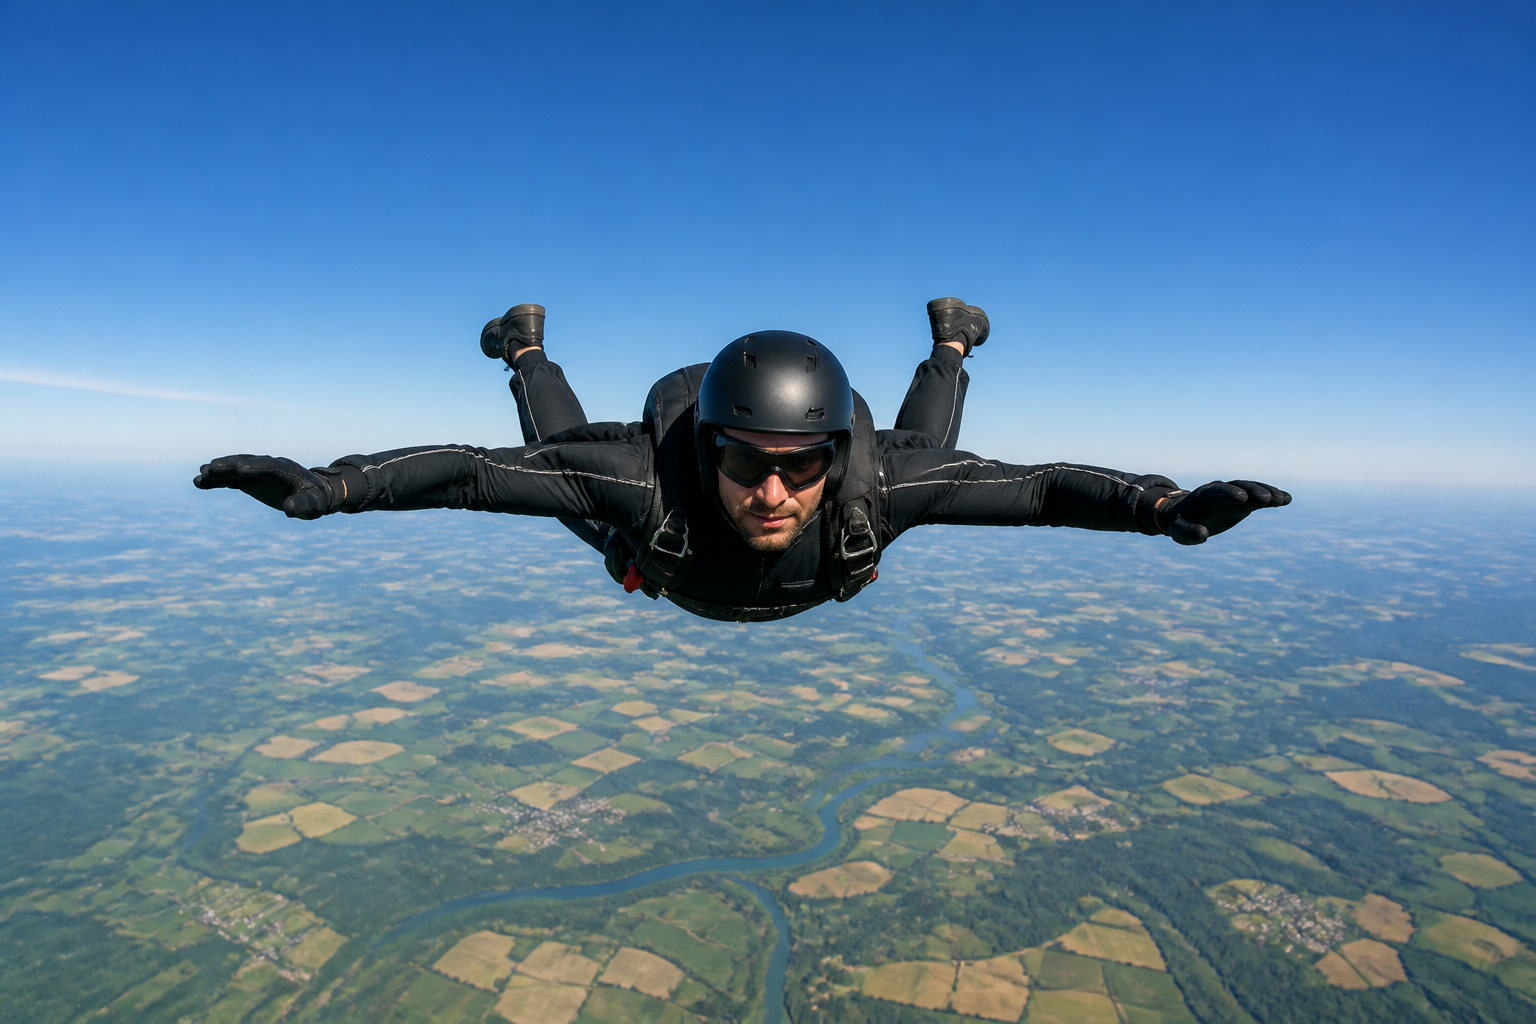
\includegraphics[width=0.60\linewidth]{images/book3/ai/b3-12-skydiver-freefall.png}

{\small Caída libre con aire: al cabo de unos segundos el arrastre cuadrático equilibra el peso y el paracaidista cae a una rapidez límite cercana a \qty{200}{km/h} --- el problema de fin de semana.}
\end{omfigure}

\section{Problema: el paracaidista}

\begin{problem}[{Problema de fin de semana --- de la puerta del avión al
suelo: caída libre, el aire que empuja de vuelta, una vela que se abre
demasiado deprisa y el aterrizaje --- una ley del movimiento, dos leyes de arrastre}]
\label{pb:b1:newton-dynamics:1}
Un paracaidista con su equipo tiene una \omterm{def:b1:newton-dynamics:momentum}{masa} $m = \qty{80}{kg}$. Aire:
$\rho = \qty{1.2}{kg/m^3}$, $\eta = \qty{1.8e-5}{Pa.s}$. Cayendo boca
abajo, $C_xS = \qty{0.80}{m^2}$; con la vela abierta, $C_xS =
\qty{25}{m^2}$. $g = \qty{9.81}{m/s^2}$; $z$ se cuenta hacia abajo desde
el punto de salto.

\medskip
\noindent\textbf{Parte I --- Sin aire.}
\begin{enumerate}
  \item Escríbase la segunda ley de Newton y dense $v(t)$ y $z(t)$;
        calcúlense ambos en $t = \qty{10}{s}$.
  \item Calcúlese el peso.
  \item El paracaidista se siente ``ingrávido'' durante esta fase aunque
        la gravedad actúe por completo. Explíquese con las \omterm{def:b1:newton-dynamics:momentum}{fuerzas} (qué
        falta respecto de estar de pie en el suelo).
  \item ¿Es el sistema terrestre bastante inercial para este problema?
        Nómbrese lo que se desprecia.
\end{enumerate}

\medskip
\noindent\textbf{Parte II --- Cayendo a través del aire.}
\begin{enumerate}[resume]
  \item Escríbase la \omterm{prop:b1:newton-dynamics:drag}{fuerza de arrastre} para la caída boca abajo en
        función de $v$.
  \item Escríbase la ecuación del movimiento para $v(t)$.
  \item Hállese la \omterm{prop:b1:newton-dynamics:terminal}{velocidad límite} $v_\infty$ (en \unit{m/s} y en
        \unit{km/h}).
  \item Con $u = v/v_\infty$ y $\tau = v_\infty/g$, muéstrese que
        $\dd u/\dd t = (1 - u^2)/\tau$; calcúlese $\tau$.
  \item Resuélvase por separación de variables y muéstrese que
        $v = v_\infty\tanh(t/\tau)$.
  \item ¿Al cabo de cuánto tiempo es $v = 0.9v_\infty$? ¿Y $0.99v_\infty$?
  \item Muéstrese que $z(t) = v_\infty\tau\ln\cosh(t/\tau)$ y calcúlese la
        distancia caída en $t = \qty{10}{s}$; compárese con la Parte I.
  \item Estímese el número de Reynolds en $v_\infty$ con $L = \qty{0.5}{m}$
        y justifíquese la ley cuadrática.
\end{enumerate}

\medskip
\noindent\textbf{Parte III --- Se abre la vela.}
\begin{enumerate}[resume]
  \item Calcúlese la nueva \omterm{prop:b1:newton-dynamics:terminal}{velocidad límite} con la vela abierta.
  \item Si la vela se abriera instantáneamente a $v = \qty{40}{m/s}$,
        ¿cuál sería la deceleración, en \unit{m/s^2} y en $g$? ¿Por qué
        resulta inaceptable?
  \item Las velas reales se abren en unos \qty{3}{s}. Estímense la
        deceleración media y la \omterm{def:b1:newton-dynamics:momentum}{fuerza} media del arnés sobre el
        paracaidista.
  \item Una vez abierta del todo la vela, la rapidez decae hacia la nueva
        $v_\infty$: ¿cuál es la nueva \omterm{def:b1:transient-regimes:firstorder}{constante de tiempo}
        $\tau' = v_\infty'/g$, y qué significa para la llegada al descenso
        estacionario?
  \item En descenso estacionario, ¿cuál es la \omterm{def:b1:newton-dynamics:momentum}{fuerza} del arnés?
        Justifíquese con la segunda ley.
  \item Explíquese por qué la \omterm{prop:b1:newton-dynamics:terminal}{velocidad límite} varía como
        $1/\sqrt{C_xS}$: ¿por qué factor la subiría una vela de la mitad
        de área?
  \item Un saltador más pesado (\qty{100}{kg}) con la misma vela:
        ¿\omterm{prop:b1:newton-dynamics:terminal}{velocidad límite}?
\end{enumerate}

\medskip
\noindent\textbf{Parte IV --- El aterrizaje.}
\begin{enumerate}[resume]
  \item La rapidez de aterrizaje es la $v_\infty$ de la vela. ¿Desde qué
        altura habría que saltar, sin aire, para llegar al suelo con esa
        rapidez?
  \item Un aterrizaje con las piernas rígidas detiene el cuerpo en
        \qty{0.5}{m}; una voltereta, en \qty{1.5}{m}. Estímense la
        deceleración media (en $g$) y la \omterm{def:b1:newton-dynamics:momentum}{fuerza} media sobre las piernas en
        cada caso, y conclúyase.
  \item Justo antes de tomar tierra, el paracaidista tira de los dos
        mandos, lo que aumenta brevemente el arrastre de la vela.
        Explíquese cualitativamente el efecto sobre la rapidez.
\end{enumerate}

\medskip
\noindent\textbf{Parte V --- Las cosas pequeñas caen de otro modo.}
\begin{enumerate}[resume]
  \item Una gota de lluvia de radio \qty{1.0}{mm} ($C_x = 0.5$):
        calcúlese su \omterm{prop:b1:newton-dynamics:terminal}{velocidad límite} con la ley cuadrática y
        compruébese el número de Reynolds.
  \item Una gotita de niebla de radio \qty{10}{\micro m}: úsese la \omterm{prop:b1:newton-dynamics:drag}{ley de
        Stokes} para $v_\infty$ y compruébese que el número de Reynolds es
        en efecto pequeño.
  \item Resúmase: una ecuación del movimiento, dos regímenes de arrastre y
        los tres números (\unit{m/s}) que deciden si algo cae como una
        piedra, como una hoja o no cae.
\end{enumerate}
\end{problem}
